\documentclass[prb,11pt,tightenlines,twocolumn,aps]{revtex4-1}

% preamble:

\usepackage{amsmath}    % need for subequations
\usepackage{graphicx}   % need for figures
\usepackage{verbatim}   % useful for program listings
\usepackage{color}      % use if color is used in text
\usepackage{subfigure}  % use for side-by-side figures
\usepackage{hyperref}   % use for hypertext links, including those to external
                        % documents and URLs 
\usepackage{blindtext}  % fill text
\usepackage{color}
\usepackage{multirow}
% \usepackage{showframe}
\usepackage[inline]{showlabels}

\raggedbottom           % don't add extra vertical space

\begin{document}

\title{Pure Spin Current Injection in Hydrogenated Graphene Structures}
\author{Reinaldo Zapata-Pe\~na\textsuperscript{1},
        Bernardo S. Mendoza\textsuperscript{1},
        Anatoli I. Shkrebtii\textsuperscript{2}}
\affiliation{\textsuperscript{1}Centro de Investigaciones en \'Optica, Le\'on,
Guanajuato 37150, M\'exico}
\affiliation{\textsuperscript{2}University of Ontario, Institute of Technology,
Oshawa, ON, L1H 7L7, Canada}

\date{\today}

\begin{abstract}
\blindtext
\end{abstract}

\maketitle

%%%%%%%%%%%%%%%%%%%%%%%%%%%%%%%%%%%%%%%%%%%%%%%%%%%%%%%%%%%%%%%%%%%%%%%%%%%%%%
%%%%%%%%%%%%%%%%%%%%%%%%%%%%%%%%%%%%%%%%%%%%%%%%%%%%%%%%%%%%%%%%%%%%%%%%%%%%%%
%%%%%%%%%%%%%%%%%%%%%%%%%%                          %%%%%%%%%%%%%%%%%%%%%%%%%%
%%%%%%%%%%%%%%%%%%%%%%%%%%  I N T R O D U C T I O N %%%%%%%%%%%%%%%%%%%%%%%%%%
%%%%%%%%%%%%%%%%%%%%%%%%%%                          %%%%%%%%%%%%%%%%%%%%%%%%%%
%%%%%%%%%%%%%%%%%%%%%%%%%%%%%%%%%%%%%%%%%%%%%%%%%%%%%%%%%%%%%%%%%%%%%%%%%%%%%%
%%%%%%%%%%%%%%%%%%%%%%%%%%%%%%%%%%%%%%%%%%%%%%%%%%%%%%%%%%%%%%%%%%%%%%%%%%%%%%

\section{Introduction}
\blindtext
\begin{figure}[ht!]
    \centering
    \subfigure[\ $xz$ plane view]
    {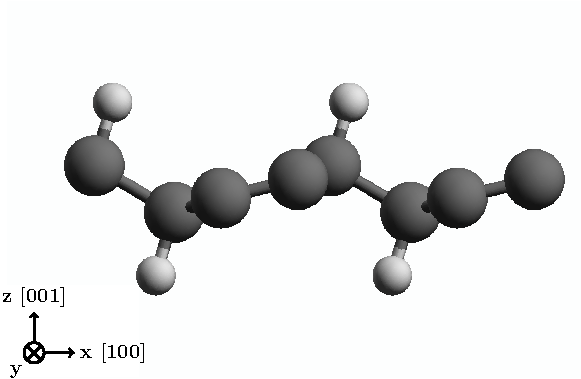
\includegraphics[width=\linewidth]{figures/altstruc2}}
    \label{fig:alt-struc-xz}
    \\
    \subfigure[\ $xy$ plane view]
    {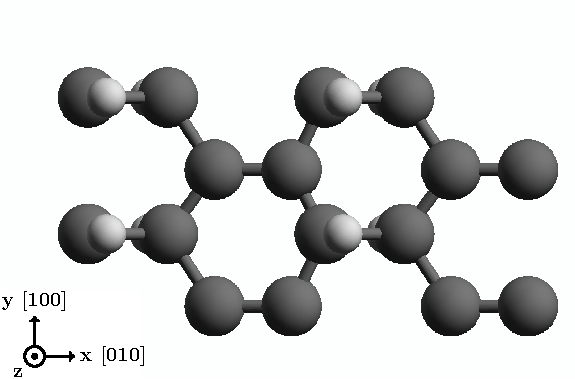
\includegraphics[width=\linewidth]{figures/altstruc1}}
    \label{fig:alt-struc-xy}
    \caption{Alt structure.}
    \label{fig:alt-struc}
\end{figure}
\begin{figure}[ht!]
    \centering
    \subfigure[\ $xz$ plane view]
    {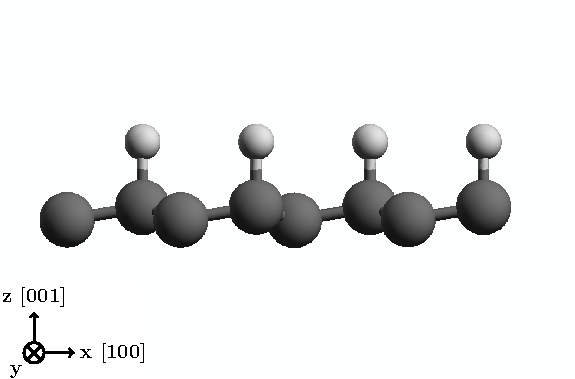
\includegraphics[width=\linewidth]{figures/upstruc2}}
    \label{fig:up-struc-xz}
    \\
    \subfigure[\ $xy$ plane view]
    {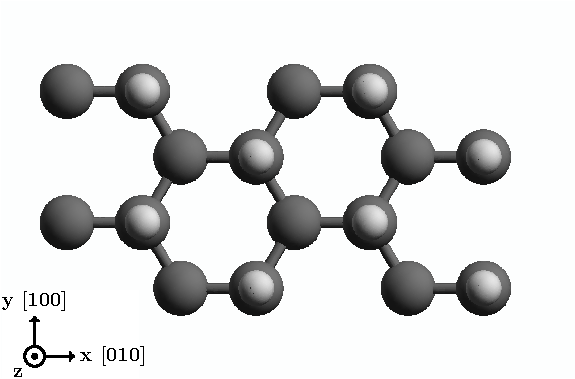
\includegraphics[width=\linewidth]{figures/upstruc1}}
    \label{fig:up-struc-xy}
    \caption{Up structure}
    \label{fig:up-struc}
\end{figure}
\blindtext
\blindtext

\blindtext

%%%%%%%%%%%%%%%%%%%%%%%%%%%%%%%%%%%%%%%%%%%%%%%%%%%%%%%%%%%%%%%%%%%%%%%%%%%%%%
%%%%%%%%%%%%%%%%%%%%%%%%%%%%%%%%%%%%%%%%%%%%%%%%%%%%%%%%%%%%%%%%%%%%%%%%%%%%%%
%%%%%%%%%%%%%%%%%%%%%%%%%%%%%%%%               %%%%%%%%%%%%%%%%%%%%%%%%%%%%%%%
%%%%%%%%%%%%%%%%%%%%%%%%%%%%%%%%  T H E O R Y  %%%%%%%%%%%%%%%%%%%%%%%%%%%%%%%
%%%%%%%%%%%%%%%%%%%%%%%%%%%%%%%%               %%%%%%%%%%%%%%%%%%%%%%%%%%%%%%%
%%%%%%%%%%%%%%%%%%%%%%%%%%%%%%%%%%%%%%%%%%%%%%%%%%%%%%%%%%%%%%%%%%%%%%%%%%%%%%
%%%%%%%%%%%%%%%%%%%%%%%%%%%%%%%%%%%%%%%%%%%%%%%%%%%%%%%%%%%%%%%%%%%%%%%%%%%%%%

\section{Theory} % (fold)
\label{sec:theory}

%%%%%%%%%%%%%%%%%%%%%%%%%%%%%%%%%%%%%%%%%%%%%%%%%%%%%%%%%%%%%%%%%%%%%%%%%%%%%%
%%%%%%%%%%%%%%%%%%%%%%%%%%% Theory: Spin velocity %%%%%%%%%%%%%%%%%%%%%%%%%%%%
%%%%%%%%%%%%%%%%%%%%%%%%%%%%%%%%%%%%%%%%%%%%%%%%%%%%%%%%%%%%%%%%%%%%%%%%%%%%%%

\subsection{Pure spin velocity} % (fold)
\label{sec:theory-pure_spin_current}

The spin density injection current $\dot{K}^{\mathrm{ab}}$ with speed along
direction $\mathrm{a}$ and spin polarization along $\mathrm{b}$ is defined as
\begin{equation}
\dot{K} = \mu^{\mathrm{abcd}}(\omega)
E^{\mathrm{c}}(\omega) E^{\mathrm{d*}}(\omega)
\label{eq:dotk}
\end{equation}
where
\begin{widetext}
\begin{equation}
\mu^{\mathrm{abcd}} (\omega) =
\frac{\pi e^{2}}{\hbar^{2}} \int 
\frac{d^{3}K}{8 \pi^{3}} \sum_{vcc'}^{'}
\mathrm{Re} \left[ K^{\mathrm{ab}}_{cc'} ( 
r^{\mathrm{c}}_{vc'} 
r^{\mathrm{d}}_{cv } +
r^{\mathrm{d}}_{vc'} 
r^{\mathrm{c}}_{cv } ) \right]
\delta(\omega-\omega_{cv})
\label{eq:mu}
\end{equation}
\end{widetext}
is the corresponding spin density injection current pseudotensor. The $'$
in the sum means that $c$ and $c'$ are quasi degenerate states and the sum only
covers these states.

Now we define the spin velocity, $\mathcal{V}^{\mathrm{ab}}$ as the speed at
which the spin polarized in the $\mathrm{b}$   direction moves along the
$\mathrm{a}$ direction when a normal incident beam reaches the $xy$ plane with a
polarization angle $\alpha$. Then,
\begin{widetext}
\begin{align}
\mathcal{V}^{\mathrm{ab}} (\omega) 
&= \frac{2}{\hbar}
\frac{\mu^{\mathrm{abxx}}(\omega)
E^{2}(\omega)\cos^{2}(\alpha) + 
\mu^{\mathrm{abyy}}(\omega)
E^{2}(\omega)\sin^{2}(\alpha) + 
2\mu^{\mathrm{abxy}}(\omega)
E^{2}(\omega)\cos(\alpha)\sin(\alpha)}
{\xi^{\mathrm{xx}}(\omega)
E^{2}(\omega)\cos^{2}(\alpha) + 
\xi^{\mathrm{yy}}(\omega)
E^{2}(\omega)\sin^{2}(\alpha)},
\nonumber \\
&= \frac{2}{\hbar}
\frac{\mu^{\mathrm{abxx}}(\omega)\cos^{2}(\alpha) + 
\mu^{\mathrm{abyy}}(\omega)\sin^{2}(\alpha) + 
\mu^{\mathrm{abxy}}(\omega)\sin(2\alpha)}
{\xi^{\mathrm{xx}}(\omega)\cos^{2}(\alpha) + 
\xi^{\mathrm{yy}}(\omega)\sin^{2}(\alpha)}.
\label{eq:vab}
\end{align}
\end{widetext}

For an angle $\alpha = \frac{\pi}{4}$ this expression can be reduced to 
\begin{align}
\mathcal{V}^{\mathrm{ab}} (\omega)
&= \frac{2}{\hbar}
\frac{\mu^{\mathrm{abxx}}(\omega) + \mu^{\mathrm{abyy}}(\omega) + 
2\mu^{\mathrm{abxy}}(\omega)}
{\xi^{\mathrm{xx}}(\omega) + \xi^{\mathrm{yy}}(\omega)}.
\label{eq:vab-90deg}
\end{align}


%%%%%%%%%%%%%%%%%%%%%%%%%%%%%%%%%%%%%%%%%%%%%%%%%%%%%%%%%%%%%%%%%%%%%%%%%%%%%%
%%%%%%%%%%%%%%%%%%%%%%%%%%%% Theory: Fixing spin %%%%%%%%%%%%%%%%%%%%%%%%%%%%%
%%%%%%%%%%%%%%%%%%%%%%%%%%%%%%%%%%%%%%%%%%%%%%%%%%%%%%%%%%%%%%%%%%%%%%%%%%%%%%

\subsection{Fixing spin}\label{sec:theory-fixspin}
Considering that we have 2D structures we can fix the spin direction along the
$x$, $y$, and $z$ Cartesian coordinates and then define the magnitude of the
spin velocity $|\mathcal{V}_{\sigma^{\mathrm{b}}}|$ in a fixed angle
$\gamma_{b}$ as
\begin{align}
|\mathcal{V}_{\sigma^{\mathrm{b}}}| (\omega)
&=
\sqrt{
(\mathcal{V}^{\mathrm{ax}}(\omega))^{2}\ +
(\mathcal{V}^{\mathrm{ay}}(\omega))^{2}\ 
}, 
\label{eq:vs-mag}
\\
\gamma_{\mathrm{b}} (\omega)
&=
\tan^{-1} \left( \frac{\mathcal{V}^{\mathrm{ay}}(\omega)}
{\mathcal{V}^{\mathrm{ax}}(\omega)} \right),
\label{eq:gamma-ang}
\end{align}
where the angle is measured in the counter-clockwise direction from the positive
$x$ axis.

%%%%%%%%%%%%%%%%%%%%%%%%%%%%%%%%%%%%%%%%%%%%%%%%%%%%%%%%%%%%%%%%%%%%%%%%%%%%%%
%%%%%%%%%%%%%%%%%%%%%%%%%%%% Theory: Fixing vel %%%%%%%%%%%%%%%%%%%%%%%%%%%%%%
%%%%%%%%%%%%%%%%%%%%%%%%%%%%%%%%%%%%%%%%%%%%%%%%%%%%%%%%%%%%%%%%%%%%%%%%%%%%%%

\subsection{Fixing velocity.}\label{sec:theory-fixvel}

In a similar way we can fix the velocity in the $xy$ plane
along $x$ and $y$ directions and define $|\mathcal{V}^{\mathrm{a}}|$ as
\begin{equation}
|\mathcal{V}^{\mathrm{a}}| (\omega)= 
\sqrt {
(\mathcal{V}^{\mathrm{ax}}(\omega))^{2} +
(\mathcal{V}^{\mathrm{ay}}(\omega))^{2} +
(\mathcal{V}^{\mathrm{az}}(\omega))^{2} 
},
\label{eq:vv-mag}
\end{equation}
and the corresponding polar and azimuthal angles $\theta$ and $\varphi$ as
\begin{align}
\theta  (\omega)
=& 
\cos^{-1} \left( \frac{\mathcal{V}^{\mathrm{az}}(\omega)}
{|\mathcal{V}^{\mathrm{a}}(\omega)|} \right),
& 0 \leq &\theta \leq \pi, 
\label{eq:polar-ang}
\\
\varphi (\omega)
=& 
\tan^{-1} \left( \frac{\mathcal{V}^{\mathrm{ay}}(\omega)}
{\mathcal{V}^{\mathrm{ax}}(\omega)} \right),
& 0 \leq &\varphi \leq 2\pi.
\label{eq:azimuthal-ang} 
\end{align}

\subsection{Layer-by-layer analysis.}\label{sec:theory-layer}

For a layered system we have that the total contribution of Eqns. 
\eqref{eq:vs-mag} and \eqref{eq:vv-mag} is given \cite{arzatePRB14} by 

\begin{align}
|\mathcal{V}_{\sigma^{\mathrm{b}}}(\omega)|
=& 
\ell_{\mathrm{eff}}
\sum_{\ell=1}^{N_{\mathrm{eff}}}
|\mathcal{V}_{\sigma^{\mathrm{b}}} (\ell | \omega)|
\label{eq:vs-layer}
\\
|\mathcal{V}^{\mathrm{a}}(\omega)|
=&
\ell_{\mathrm{eff}}
\sum_{\ell=1}^{N_{\mathrm{eff}}}
|\mathcal{V}^{\mathrm{a}} (\ell | \omega)|
\label{eq:vv-layer}
\end{align}



%%%%%%%%%%%%%%%%%%%%%%%%%%%%%%%%%%%%%%%%%%%%%%%%%%%%%%%%%%%%%%%%%%%%%%%%%%%%%%
%%%%%%%%%%%%%%%%%%%%%%%%%%%%%%%%%%%%%%%%%%%%%%%%%%%%%%%%%%%%%%%%%%%%%%%%%%%%%%
%%%%%%%%%%%%%%%%%%%%%%%%%%%%%                   %%%%%%%%%%%%%%%%%%%%%%%%%%%%%%
%%%%%%%%%%%%%%%%%%%%%%%%%%%%%   R E S U L T S   %%%%%%%%%%%%%%%%%%%%%%%%%%%%%%
%%%%%%%%%%%%%%%%%%%%%%%%%%%%%                   %%%%%%%%%%%%%%%%%%%%%%%%%%%%%%
%%%%%%%%%%%%%%%%%%%%%%%%%%%%%%%%%%%%%%%%%%%%%%%%%%%%%%%%%%%%%%%%%%%%%%%%%%%%%%
%%%%%%%%%%%%%%%%%%%%%%%%%%%%%%%%%%%%%%%%%%%%%%%%%%%%%%%%%%%%%%%%%%%%%%%%%%%%%%

\section{Results} % (fold)
\label{sec:results}

\begin{table}[t]
\center
\begin{tabular}{ccccc}\\
\hline
\quad Layer \quad & \quad Atom \qquad & \multicolumn{3}{c}{Position [\AA]} \\
\cline{3-5}
\quad No.   \quad & \quad type \qquad & $x$ & $y$ & $z$  \\
\hline
1 & H &  -0.61516 &  -1.42140 & \ 1.47237 \\
2 & C &  -0.61516 &  -1.73300 & \ 0.39631 \\
3 & C & \ 0.61516 & \ 1.73300 & \ 0.15807 \\
4 & C & \ 0.61516 & \ 0.42201 &  -0.15814 \\
5 & C &  -0.61516 &  -0.37396 &  -0.39632 \\
6 & H &  -0.61516 &  -0.68566 &  -1.47237 \\
\hline
\end{tabular}
\caption{Unit cell of \emph{alt} structure. Layer division, atom types and
positions for the \emph{alt} structure. The structure unit cell was divided in
six layers corresponding each one to atoms in different $z$ positions. The
corresponding layer atom position is depicted in Fig. \ref{fig:alt-struc} with
the corresponding number of layer.}
\label{tab:alt-unitcell}
\end{table}
% 
\begin{table}[t]
\center
\begin{tabular}{ccccc}\\
\hline
\quad Layer \quad & \quad Atom \qquad & \multicolumn{3}{c}{Position [\AA]} \\
\cline{3-5}
\quad No.   \quad & \quad type \qquad & $x$ & $y$ & $z$  \\
\hline
1 & H & -0.61516 & -1.77416 &  0.73196 \\
1 & H &  0.61518 &  0.35514 &  0.73175 \\
2 & C & -0.61516 & -1.77264 & -0.49138 \\
2 & C & -0.61516 & -0.35600 & -0.72316 \\
2 & C &  0.61516 &  0.35763 & -0.49087 \\
\hline
\end{tabular}
\caption{Unit cell of \emph{up} structure. Layer division, atom types and
positions for the \emph{up} structure. The structure unit cell was divided in
two layers corresponding to hydrogen and carbon atoms.The corresponding layer
atom position is depicted in Fig. \ref{fig:up-struc} with the corresponding
number of layer.}
\label{tab:up-unitcell}
\end{table}

We preset the results for $\mathcal{V}^{\mathrm{ab}}$ for the
C$_{16}$H$_{8}$-alt and C$_{16}$H$_{8}$-up structures being both
noncentrosymmetric semi-infinite carbon systems with 50\% hydrogenation in
different arrangements. The \emph{alt} system has alternating hydrogen atoms on
the upper and bottom sides of the carbon sheet, while the \emph{up} system has H
only on the upper side. We take the hexagonal carbon lattice to be on the $xy$
plane for both structures, and the carbon-hydrogen bonds on the perpendicular
$xz$ plane, as depicted in Figs.
\ref{fig:alt-struc} and \ref{fig:up-struc}.

Using the ABINIT code \cite{gonzeCPC09} we calculated the self- consistent
ground state and the Kohn-Sham states using density functional theory in the
local density approximation (DFT-LDA) with a planewave basis. We used
Hartwigsen- Goedecker-Hutter (HGH) relativistic separable dual-space Gaussian
pseudopotentials \cite{hartwigsenPRB98} including the spin-orbit interaction
for calculating $\mathcal{V}^{\mathrm{a}}(\omega)$.

The convergence parameters for the calculations of our results corresponding to
the \emph{alt} and \emph{up} structures are cutoff energies of 65\,Ha and
40\,Ha, respectively. The energy eigenvalues and matrix elements were
calculated using 14452 $\mathbf{k}$ points and 8452 $\mathbf{k}$ points in the
irreducible Brillouin zone (IBZ) and present LDA energy band gaps of 0.72\,eV
and 0.088\,eV, respectively for the \emph{alt} and \emph{up} structures. As
mentioned in
\cite{zapataPSB2016}, using DFT the LDA is only one method of many other that
can be used to calculate the electronic structure of materials. Also it is
known that all methods predict a different band gap than the obtained in the
experiment. A correction for the band gap energy value can be calculated by
other \emph{ab-initio} methods such as the GW approximation \cite{onidaRMP02}
being this outside the scope of this paper.

The structures presented here where divided into layers to analyze the he
layer-by-layer contribution for $\mathcal{V}^{\mathrm{ab}}$ response. The
\emph{alt} structure was divided in six layers corresponding the first one to
the top hydrogen atoms, from the second to the forth to carbon atoms in
different $z$ positions, and the sixth and last one to the bottom hydrogen
atoms. The \emph{up} structure was divided into two layers, the first one
comprised by the top hydrogen atoms and the second by the carbon atoms. The
layer divisions and atom positions for the unit cells are shown in Tables
\ref{tab:alt-unitcell} and \ref{tab:up-unitcell}.


%%%%%%%%%%%%%%%%%%%%%%%%%%%%%%%%%%%%%%%%%%%%%%%%%%%%%%%%%%%%%%%%%%%%%%%%%%%%%%
%%%%%%%%%%%%%%%%%%%%%%%%%%% Results: Spin velocity %%%%%%%%%%%%%%%%%%%%%%%%%%%
%%%%%%%%%%%%%%%%%%%%%%%%%%%%%%%%%%%%%%%%%%%%%%%%%%%%%%%%%%%%%%%%%%%%%%%%%%%%%%


\subsection{Spin velocity} % (fold)
\label{sec:res-pure_spin_current_and_spin_velocity}

%%%%%%%%%%%%%%%%%%%%%%%%%%%%%%%%%%%%%%%%%%%%%%%%%%%%%%%%%%%%%%%%%%%%%%%%%%%%%%
%%%%%%%%%%%%%%%%%%%%%%%%%% Res: mu & V^{ab} comparison %%%%%%%%%%%%%%%%%%%%%%%

\begin{figure}[t]
    \centering
    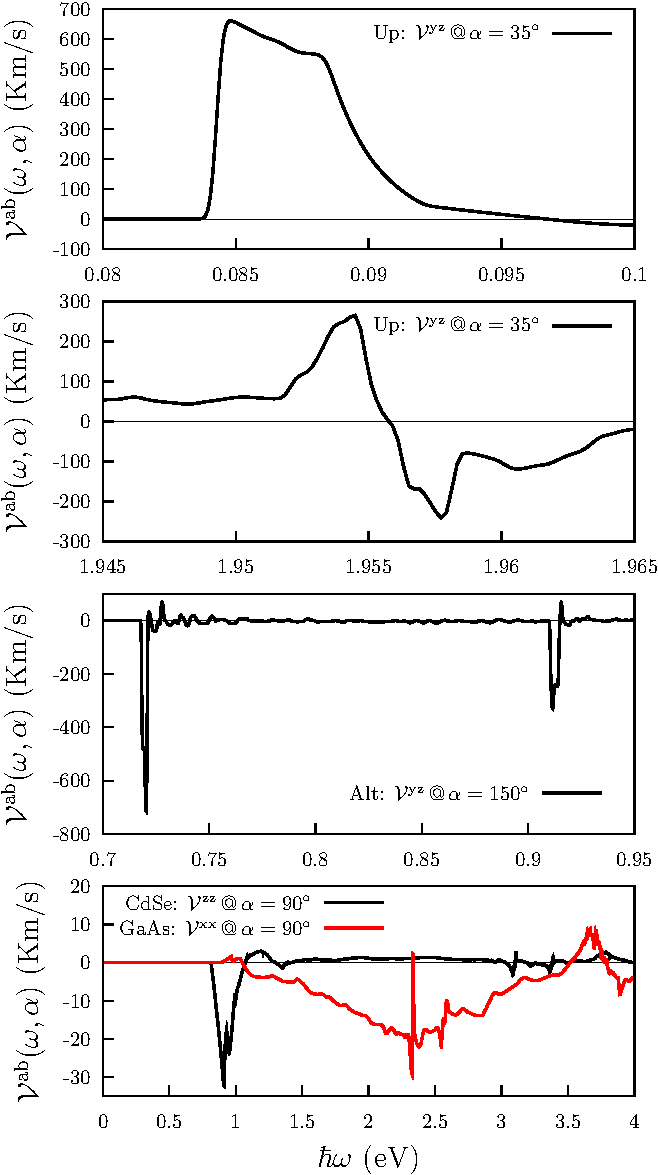
\includegraphics[width=\linewidth]{plots/vab-str-comp}
    \caption{Comparison of most intense responses for
    $\mathcal{V}^{\mathrm{ab}}$ for \emph{alt}, \emph{up}, CdSe, and GaAs
    structures}
    \label{fig:vab-str-comp}
\end{figure}

In figure \ref{fig:vab-str-comp} we present a comparison of the most intense
responses resulting from evaluate the Eq. \eqref{eq:vab} for the \emph{alt} and
\emph{up} 2D structures vs. CdSe and GaAs bulk structures. As we can see from
this figure the most intense response corresponds to the \emph{up} structure
centered at 0.088\,eV corresponding to the terahertz radiation and reaching a
spin velocity of 87.16\,Km/s.
% 
In the other hand, for an energy range from 0.66\,eV to 3.0\,eV all the
four structures have contributions in the same order of magnitude. 
% 
Starting with the 2D structures we have that the \emph{up} structure has other
two peaks centered at 1.94\,eV and 1.97\,eV reaching spin velocities of
22.2\,Km/s and -29.7\,Km/s, respectively, and the \emph{alt} structure has two
peaks centered at 0.72\,eV and 0.91\,eV reaching spin velocities of -40.2\,Km/s
and -32.9\,Km/s, respectively.
% 
Then, for the bulk structures we have that the CdSe has only one intense
response centered at 0.91\,eV reaching a spin velocity of -26.9\,Km/s, and the
GaAs structure has a large and almost planar zone where the response is hold
reaching the maximum for an incoming beam of energy of 2.31\,eV and reaching a
spin velocity of -21.6\,Km/s.
% 
In table \ref{tab:vab-str-comp} we present the comparison of this values for the 2D and bulk structures.
% 
\begin{table}[t]
\begin{tabular}{cccccc}
\hline
\hline
Kind of  & 
\multirow{2}{*}{\quad Structure \quad} & 
Pol. &
Energy & 
\multicolumn{2}{c}{$\mathcal{V}^{\mathrm{ab}}(\omega)$}\\
\cline{5-6}
system & & Ang. & [eV] & $\mathrm{ab}$ \quad & [Km/s]\\
\hline
\hline
2D   & \emph{up}    & 40    & 0.09  & $\mathrm{yz}$ &  87.16    \\
     &              &       & 1.94  & $\mathrm{yz}$ &  22.22    \\
     &              &       & 1.97  & $\mathrm{yz}$ & -29.70    \\
\hline
2D   & \emph{alt}   & 145   & 0.72  & $\mathrm{yz}$ & -40.21    \\
     &              &       & 0.91  & $\mathrm{yz}$ & -32.89    \\
\hline
bulk &  CdSe        & 90    & 0.91  & $\mathrm{zz}$ & -26.87    \\
\hline
bulk &  GaAs        & 90    & 2.31  & $\mathrm{xx}$ & -21.62    \\
\hline
\hline
\end{tabular}
\caption{Comparison of the reported maxima values of $\mathcal{V}^{\mathrm{ab}}$
for different structures and the corresponding polarization angle $\alpha$ and
energy values.}
\label{tab:vab-str-comp}
\end{table}


%%%%%%%%%%%%%%%%%%%%%%%%%%%%%%%%%%%%%%%%%%%%%%%%%%%%%%%%%%%%%%%%%%%%%%%%%%%%%%
%%%%%%%%%%%%%%%%%%%%%%%%%%%% Results: Fixing spin %%%%%%%%%%%%%%%%%%%%%%%%%%%%
%%%%%%%%%%%%%%%%%%%%%%%%%%%%%%%%%%%%%%%%%%%%%%%%%%%%%%%%%%%%%%%%%%%%%%%%%%%%%%

\subsection{Fixing spin} % (fold)
\label{sec:res-fixspin}

%%%%%%%%%%%%%%%%%%%%%%%%%%%%%%%%%%%%%%%%%%%%%%%%%%%%%%%%%%%%%%%%%%%%%%%%%%%%%%
%%%%%%%%%%%%%%%%%%%%%%%%%%% Res: fixing spin Up  %%%%%%%%%%%%%%%%%%%%%%%%%%%%%

\blindtext
\blindtext

%%%%%%%%%%%%%%%%%%%%%%%%%%%%%%%%%%%%%%%%%%%%%%%%%%%%%%%%%%%%%%%%%%%%%%%%%%%%%%
%%%%%%%%%%%%%%%%%%%%%%%%%% Results: Fixing velocity %%%%%%%%%%%%%%%%%%%%%%%%%%
%%%%%%%%%%%%%%%%%%%%%%%%%%%%%%%%%%%%%%%%%%%%%%%%%%%%%%%%%%%%%%%%%%%%%%%%%%%%%%

\subsection{Fixing velocity} % (fold)
\label{sec:res-fixvel}


%%%%%%%%%%%%%%%%%%%%%%%%%%%%%%%%%%%%%%%%%%%%%%%%%%%%%%%%%%%%%%%%%%%%%%%%%%%%%%
%%%%%%%%%%%%%%%%%%%%%%%%%%% Res: fixin vel Up  %%%%%%%%%%%%%%%%%%%%%%%%%%%%%%%
\textbf{Up structure.}

% %%%%%%%%%%%%%%%%%
% %% 0.0 eV - 0.16 eV
% %% Description of UP |V^{a}| 3D
% %% files: 
% %% magv.sm_0.03_xb_12802_40-spin_scissor_0_Nc_32_incang_0-180-step5
% %% magv.sm_0.03_yb_12802_40-spin_scissor_0_Nc_32_incang_0-180-step5
% %% up-3d-vab.gp
% %%%%%%%%%%%%%%%%%
\begin{figure}[t]
    \centering
    \subfigure[\ $|\mathcal{V}^{\mathrm{x}}|$ for \emph{up} structure 
    \label{fig:up-3d-vx-1}]
    {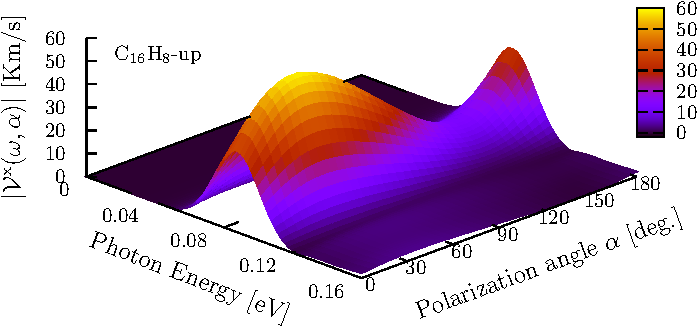
\includegraphics[width=\linewidth]{upplots/up-3d-vxb-1}}
    \\
    \subfigure[\ $|\mathcal{V}^{\mathrm{y}}|$ for \emph{up} structure 
    \label{fig:up-3d-vy-1}]
    {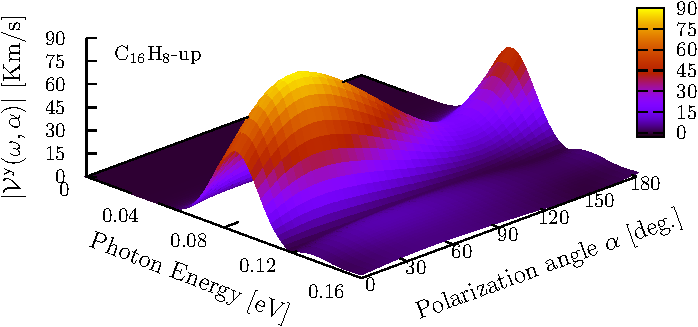
\includegraphics[width=\linewidth]{upplots/up-3d-vyb-1}}
    \caption{$|\mathcal{V}^{\mathrm{x}}|$ response for C$_{16}$H$_{8}$-up
    structure. The maximum response zone is localized for an energy range from
    0.04\,eV to 0.12\,eV and for a polarization angle of the
    incoming beam from 25$^{\circ}$ to 50$^{\circ}$.}
    \label{fig:up-3d-1}
\end{figure}
\begin{figure}[t]
    \centering
    \subfigure[\ $|\mathcal{V}^{\mathrm{x}}|$ \label{fig:up-vx-comp-rtp-1}]
    {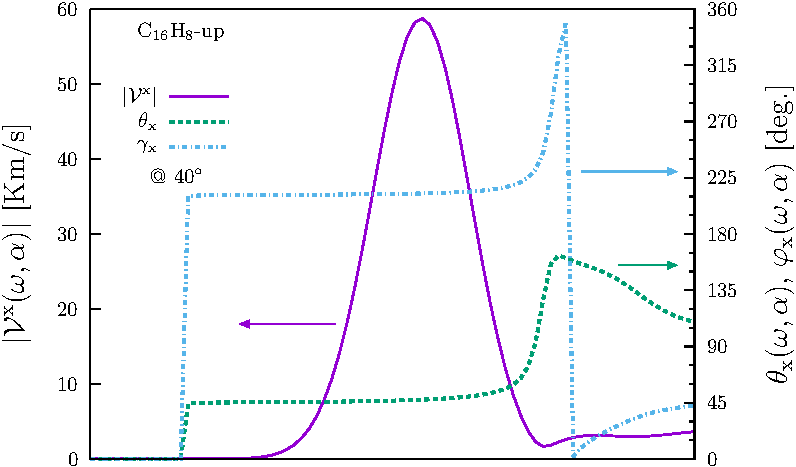
\includegraphics[width=\linewidth]{upplots/up-vxb-rtp-m1}}
    \\
    \subfigure[\ $|\mathcal{V}^{\mathrm{y}}|$ \label{fig:up-vy-comp-rtp-1}]
    {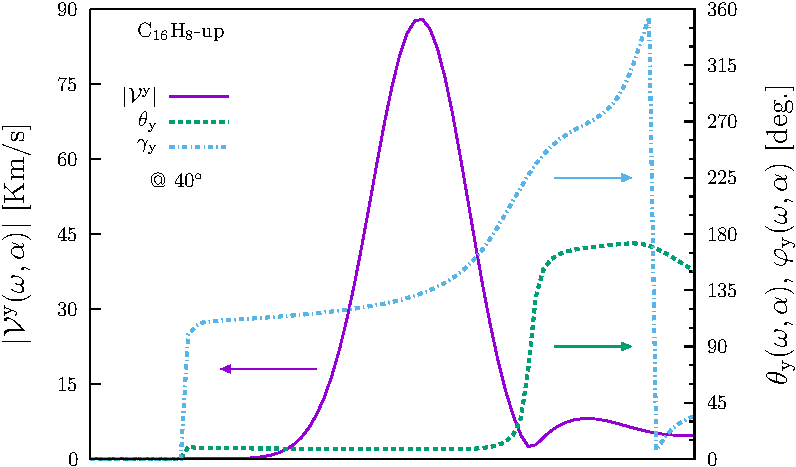
\includegraphics[width=\linewidth]{upplots/up-vyb-rtp-m1}}
    \caption{Most intense responses of $|\mathcal{V}^{\mathrm{x}}|$ and
    $|\mathcal{V}^{\mathrm{y}}|$ and the corresponding three components for the
    \emph{up} structure. Both maxima where obtained for a polarization
    angle $\alpha=40^{\circ}$. }
    \label{fig:up-vab-comp-rtp-1}
\end{figure}

For the \emph{up} structure we first analyzed the energy range from 0.00\,eV to
0.16\,eV where we found the most intense response for $\mathcal{V}^{\mathrm{x}}$
and $|\mathcal{V}^{\mathrm{y}}|$. In Fig. \ref{fig:up-3d-1} we present the
$\mathcal{V}^{\mathrm{a}}$ spectra resulting from evaluate again Eq. 
\eqref{eq:vv-mag} using different polarization angles $\alpha$ in Eq.  
\eqref{eq:vab} but now for the C$_{16}$H$_{8}$-up structure. We can see that the
onset of the response is when the energy of the incoming light is the same of
the gap energy.
% 
From this picture we can see that for the zone between the energy range of
0.084\,eV-0.093\,eV and polarization angles between $30^{\circ}$ and
$45^{\circ}$ is the zone where the maximum zone of response for both,
$|\mathcal{V}^{\mathrm{x}}|$ and $|\mathcal{V}^{\mathrm{y}}|$ is hold.
% 
We found that the absolute maximum of the response is obtained when the
polarization angle is $\alpha=40^{\circ}$ and the energy of the incoming beam is
0.088\,eV.
%
In the top frames of  Figs. \ref{fig:up-vx-comp-rtp-1} and 
% 
\ref{fig:up-vy-comp-rtp-1} we present the results of
$|\mathcal{V}^{\mathrm{x}}|$ and $|\mathcal{V}^{\mathrm{y}}|$ (left scale)
fixing the polarization angle to $\alpha=40^{\circ}$ for the \emph{up} structure
vs photon energy and the corresponding polar $\varphi$ and azimuthal $\theta$
angles (right scale). In the bottom frames of same figures we present the decomposition of
$|\mathcal{V}^{\mathrm{x}}|$ and $|\mathcal{V}^{\mathrm{y}}|$ in the
corresponding $\mathcal{V}^{\mathrm{xx}}$, 
$\mathcal{V}^{\mathrm{xy}}$,
$\mathcal{V}^{\mathrm{xz}}$, and
$\mathcal{V}^{\mathrm{yx}}$, 
$\mathcal{V}^{\mathrm{yy}}$,
$\mathcal{V}^{\mathrm{yz}}$ 
components with $\alpha$ fixed to $40^{\circ}$. 
\begin{figure}[t]
    \centering
    \subfigure[\ $|\mathcal{V}^{\mathrm{x}}|$ for \emph{up} structure 
    \label{fig:up-3d-vx-2}]
    {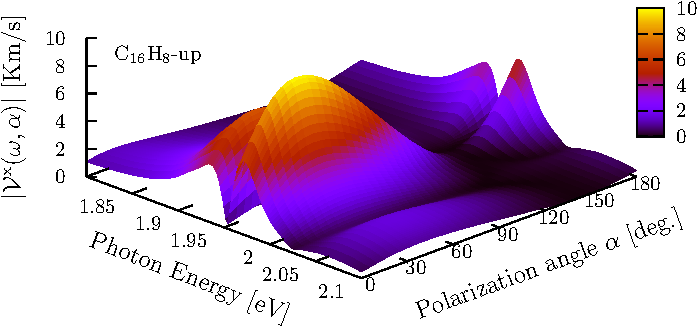
\includegraphics[width=\linewidth]{upplots/up-3d-vxb-2}}
    \\
    \subfigure[\ $|\mathcal{V}^{\mathrm{y}}|$ for \emph{up} structure 
    \label{fig:up-3d-vy-2}]
    {
\includegraphics[width=\linewidth]{upplots/up-3d-vyb-2}}
    \caption{$|\mathcal{V}^{\mathrm{x}}|$ and $|\mathcal{V}^{\mathrm{y}}|$
    response for C$_{16}$H$_{8}$-up structure. The local maxima responses zones
    are localized for an energy range from 1.95\,eV to 2.00\,eV and for
    polarization angles of the incoming beam from 25$^{\circ}$ to 50$^{\circ}$.}
    \label{fig:up-3d-2}
\end{figure}

\begin{figure}[t]
    \centering
    \subfigure[\ $|\mathcal{V}^{\mathrm{x}}|$ \label{fig:up-vx-comp-rtp-2}]
    {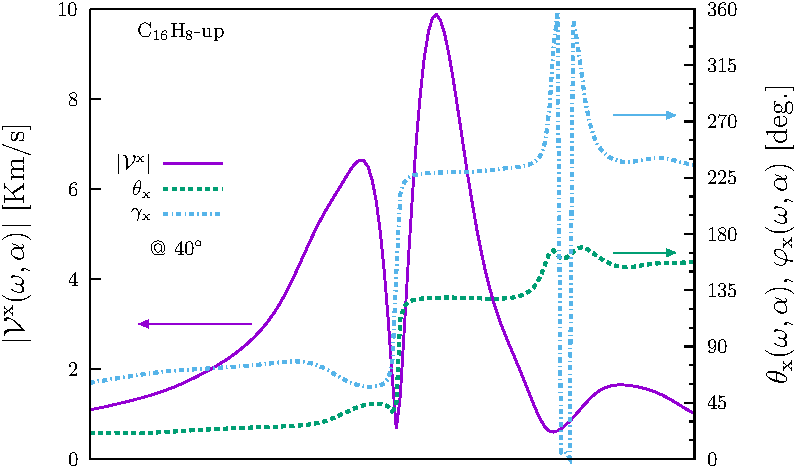
\includegraphics[width=\linewidth]{upplots/up-vxb-rtp-m2}}
    \\
    \subfigure[\ $|\mathcal{V}^{\mathrm{y}}|$ \label{fig:up-vy-comp-rtp-2}]
    {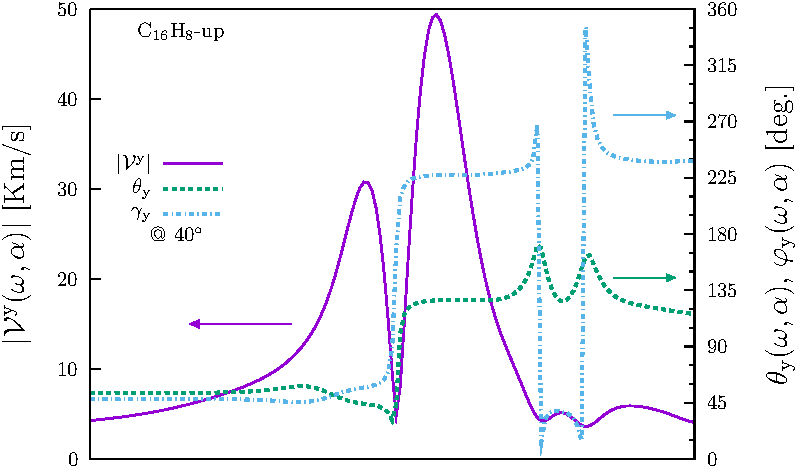
\includegraphics[width=\linewidth]{upplots/up-vyb-rtp-m2}}
    \caption{Intense responses of $|\mathcal{V}^{\mathrm{x}}|$ and
    $|\mathcal{V}^{\mathrm{y}}|$ and the corresponding three components for the
    \emph{up} structure. Both maxima where obtained for a polarization
    angle $\alpha=40^{\circ}$. }
    \label{fig:up-vab-comp-rtp-2}
\end{figure}
% %%%%%%%%%%%%%%%%%
% %% 1.8 eV - 2.0 eV
% %% Description of UP |V^{a}|, components and RTP
% %% files: 
% %% vab-rtp.sm_0.03_x_12802_40-spin_scissor_0_Nc_32_ang_040
% %% vab-rtp.sm_0.03_y_12802_40-spin_scissor_0_Nc_32_ang_040
% %% up-3d-vab.gp
% %%%%%%%%%%%%%%%%%
From Fig. \ref{fig:up-vx-comp-rtp-1} we have that for an incoming bean with
energy of 0.088\,eV the three components have similar contributions and have
values of 
% 
$\mathcal{V}^{\mathrm{xx}}=-36.5$\,Km/s,
$\mathcal{V}^{\mathrm{xy}}=-23.2$\,Km/s, and
$\mathcal{V}^{\mathrm{xz}}= 39.8$\,Km/s 
% 
resulting in a value of
% 
$|\mathcal{V}^{\mathrm{x}}|=58.7$\,Km/s 
% 
being this value the absolute maximum obtained when the spin-velocity is fixed
in the $x$ direction. To this value corresponds a polar and azimuthal angles of
$\varphi=47.4$ and $\theta=212.5$, respectively.
% 
Now, from Fig. \ref{fig:up-vy-comp-rtp-1} we have that the $yx$ and $yy$
components have less contributions for the total response than the $yz$ and for
the same incoming beam energy have values of 
% 
$\mathcal{V}^{\mathrm{yx}}= -7.9$\,Km/s 
$\mathcal{V}^{\mathrm{yy}}=  8.6$\,Km/s, and
$\mathcal{V}^{\mathrm{yz}}= 87.2$\,Km/s 
% 
resulting in a value of the total response of
% 
$|\mathcal{V}^{\mathrm{y}}|=87.9$\,Km/s
% 
being this value the absolute maximum obtained when the spin-velocity is fixed
in the $y$ direction and being 1.5 times more intense than
$|\mathcal{V}^{\mathrm{x}}|$ and corresponding spin polar and azimuthal angles
$\varphi=7.6$ $\theta=132.7$, respectively. We also found that since the onset
of the response till an energy for the incoming beam of 0.118\,eV the components
of both, $|\mathcal{V}^{\mathrm{x}}|$ and $|\mathcal{V}^{\mathrm{y}}|$ have no
change in the spin polarization direction. Finally, after this energy value both
goes to zero.
% %%%%%%%%%%%%%%%%%
% %% 1.80 eV - 2.10 eV
% %% Description of UP |V^{a}| 3D
% %% files: 
% %% magv.sm_0.03_xb_12802_40-spin_scissor_0_Nc_32_incang_0-180-step5
% %% magv.sm_0.03_yb_12802_40-spin_scissor_0_Nc_32_incang_0-180-step5
% %% up-3d-vab.gp
% %%%%%%%%%%%%%%%%%
Also there is another energy range of interest for an incoming energy beam from
1.80\,eV to 2.10\,eV presented in Fig. \ref{fig:up-3d-2} where two local maxima
of $|\mathcal{V}^{\mathrm{x}}|$ and $|\mathcal{V}^{\mathrm{y}}|$ are obtained
for the \emph{up} structure resulting from evaluate Eqns. \eqref{eq:vv-mag} and
\eqref{eq:vab}.
% 
From this figure we have that for the zone between the energy ranges from
1.92\,eV to 1.94\,eV and from 1.96\,eV to 1.98\,eV and angles from $30^{\circ}$
to $45^{\circ}$ those maxima zones are hold. 
% 
We found that the maxima are obtained when the polarization angle is fixed to
$40^{\circ}$ and the corresponding energies are 1.934\,eV and 1.972\,eV.
% 
Again, in the top frames of Figs. \ref{fig:up-vx-comp-rtp-2} and 
% 
\ref{fig:up-vy-comp-rtp-2} we present the results of
$|\mathcal{V}^{\mathrm{x}}|$ and $|\mathcal{V}^{\mathrm{y}}|$ (left scale)
fixing the polarization angle to $\alpha=40^{\circ}$ vs the photon energy and
the corresponding polar $\varphi$ and azimuthal $\theta$ angles (right scale)
for the \emph{up} structure. In the bottom frames of same figures we present the
three components $\mathrm{xx}$, $\mathrm{xy}$, $\mathrm{xz}$, and $\mathrm{yx}$,
$\mathrm{yy}$, $\mathrm{yz}$ corresponding to $|\mathcal{V}^{\mathrm{x}}|$ and
$|\mathcal{V}^{\mathrm{y}}|$ fixing the polarization angle to $40^{\circ}$.
% %%%%%%%%%%%%%%%%
% %% Starting description of UP |V^{x}|, components and RTP
% %% files: vab-rtp.sm_0.03_x_12802_40-spin_scissor_0_Nc_32_ang_040
% %%        vab-rtp.sm_0.03_y_12802_40-spin_scissor_0_Nc_32_ang_040
% %%        alt-plots/up-vab-rtp.gp
% %%%%%%%%%%%%%%%%
We found that for both cases, $|\mathcal{V}^{\mathrm{x}}|$ and
$|\mathcal{V}^{\mathrm{y}}|$, the corresponding components have similar
contributions and for an incoming energy beam of 1.934\,eV have values of
% 
$\mathcal{V}^{\mathrm{xx}}= 2.3$\,Km/s, 
$\mathcal{V}^{\mathrm{xy}}= 3.8$\,Km/s, 
$\mathcal{V}^{\mathrm{xz}}= 4.9$\,Km/s, and
$\mathcal{V}^{\mathrm{yx}}=11.5$\,Km/s,
$\mathcal{V}^{\mathrm{yy}}=17.0$\,Km/s,
$\mathcal{V}^{\mathrm{yz}}=20.4$\,Km/s
resulting in a in values of 
$|\mathcal{V}^{\mathrm{x}}|= 6.6$\,Km/s
$|\mathcal{V}^{\mathrm{y}}|=28.7$\,Km/s
% 
being $|\mathcal{V}^{\mathrm{y}}|$ 4.3 times more intense than
$|\mathcal{V}^{\mathrm{x}}|$ for this photon energy. The responses have polar
and azimuthal spin polarization angels $\varphi= 42.0^{\circ}$ and $\theta=
58.7^{\circ}$ for $|\mathcal{V}^{\mathrm{x}}|$ and $\varphi= 45.2^{\circ}$ and
$\theta= 56.0^{\circ}$ for $|\mathcal{V}^{\mathrm{y}}|$.
% 
Alike, for an incoming energy beam of 1.972\,eV all the components of
$|\mathcal{V}^{\mathrm{x}}|$ and $|\mathcal{V}^{\mathrm{y}}|$ have similar
contributions having values of
% 
$\mathcal{V}^{\mathrm{xx}}= -5.0$\,Km/s, 
$\mathcal{V}^{\mathrm{xy}}= -5.8$\,Km/s, 
$\mathcal{V}^{\mathrm{xz}}= -6.2$\,Km/s, and
$\mathcal{V}^{\mathrm{yx}}=-26.8$\,Km/s,
$\mathcal{V}^{\mathrm{yy}}=-28.9$\,Km/s,
$\mathcal{V}^{\mathrm{yz}}=-29.7$\,Km/s
resulting in a in values of 
$|\mathcal{V}^{\mathrm{x}}|= 9.9$\,Km/s
$|\mathcal{V}^{\mathrm{y}}|=49.4$\,Km/s
% 
being $|\mathcal{V}^{\mathrm{y}}|$ 5.0 times more intense than
$|\mathcal{V}^{\mathrm{x}}|$ for this photon energy. The responses have polar
and azimuthal spin polarization angles $\varphi=129.0^{\circ}$
$\theta=229.1^{\circ}$ or $|\mathcal{V}^{\mathrm{x}}|$ and
$\varphi=127.0^{\circ}$ and $\theta= 227.1^{\circ}$ for
$|\mathcal{V}^{\mathrm{y}}|$.
% 
Finally we have that all the tree components of $|\mathcal{V}^{\mathrm{x}}|$ and
$|\mathcal{V}^{\mathrm{y}}|$ keep the spin polarization positive till an energy
of the incoming beam equal to 1.954\,eV when the spin polarization changes the
direction and after an energy for the incoming beam equal to 2.05\,eV both
responses goes to zero.

%%%%%%%%%%%%%%%%%%%%%%%%%%%%%%%%%%%%%%%%%%%%%%%%%%%%%%%%%%%%%%%%%%%%%%%%%%%%%%
%%%%%%%%%%%%%%%%%%%%%%%%%%% Res: fixin vel Alt  %%%%%%%%%%%%%%%%%%%%%%%%%%%%%%%

\textbf{Alt structure.}
% %%%%%%%%%%%%%%%%%
% %% Description of ALT |V^{a}| 3D
% %% files: 
% %% magv.sm_0.03_xb_14452_65-spin_scissor_0_Nc_32_incang_0-180-step5
% %% magv.sm_0.03_yb_14452_65-spin_scissor_0_Nc_32_incang_0-180-step5
% %% alt-3d-vab.gp
% %%%%%%%%%%%%%%%%%
\begin{figure}[tb]
    \centering
    \subfigure[\ $|\mathcal{V}^{\mathrm{x}}|$ for \emph{alt} structure 
    \label{fig:alt-3d-vx}]
    {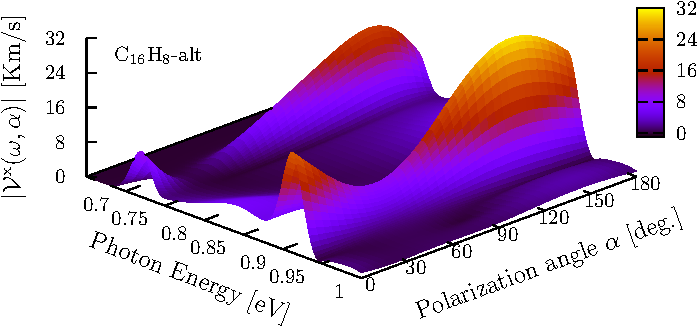
\includegraphics[width=\linewidth]{altplots/alt-3d-vxb}}
    \\
    \subfigure[\ $|\mathcal{V}^{\mathrm{y}}|$ for \emph{alt} structure 
    \label{fig:alt-3d-vy}]
    {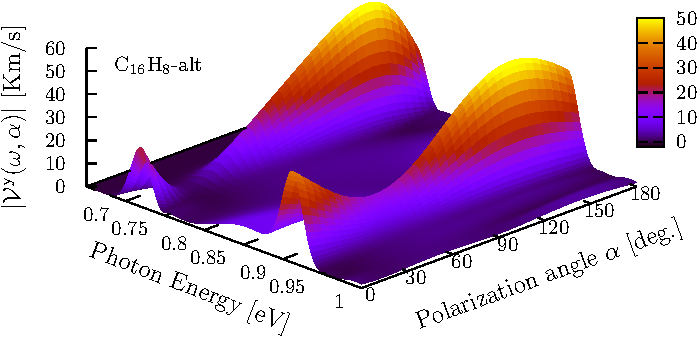
\includegraphics[width=\linewidth]{altplots/alt-3d-vyb}}
    \caption{$|\mathcal{V}^{\mathrm{x}}|$ and $|\mathcal{V}^{\mathrm{y}}|$
    responses for C$_{16}$H$_{8}$-alt structure. The maxima responses zones are
    localized for an energy range from 0.90\,eV to 0.93\,eV and for polarization
    angles of the incoming beam from 120$^{\circ}$ to 150$^{\circ}$.}
    \label{fig:alt-3d}
\end{figure}

\begin{figure}[tb]
    \centering
    \subfigure[\ $|\mathcal{V}^{\mathrm{x}}|$ \label{fig:alt-vx-comp-rtp}]
    {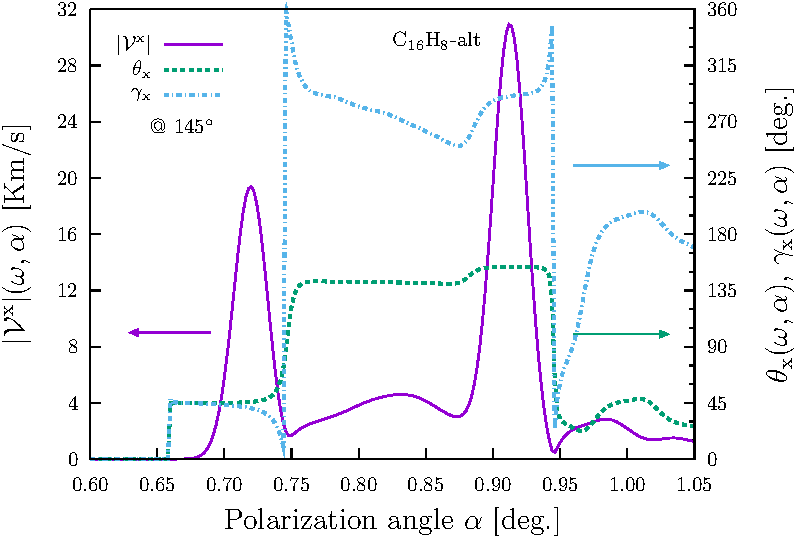
\includegraphics[width=\linewidth]{altplots/alt-vxb-rtp-m}}
    \\
    \subfigure[\ $|\mathcal{V}^{\mathrm{y}}|$ \label{fig:alt-vy-comp-rtp}]
    {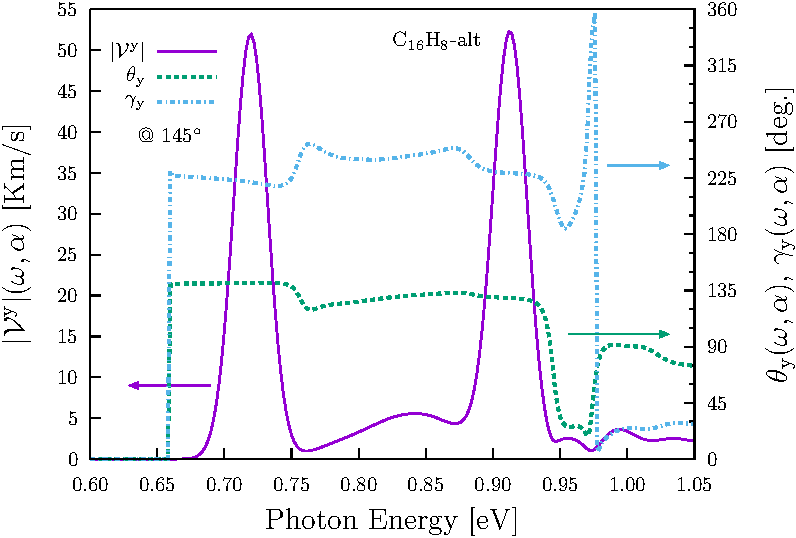
\includegraphics[width=\linewidth]{altplots/alt-vyb-rtp-m}}
    \caption{Most intense responses of $|\mathcal{V}^{\mathrm{x}}|$ and
    $|\mathcal{V}^{\mathrm{y}}|$ and the corresponding three components for the
    \emph{alt} structure. Both maxima where obtained for a polarization
    angle $\alpha=145^{\circ}$. }
    \label{fig:alt-vab-comp-rtp}
\end{figure}

For the \emph{alt} structure we analyzed the energy range from 0.6\,eV to
1.0\,eV where we found the most intense response for 
$|\mathcal{V}^{\mathrm{x}}|$ and $|\mathcal{V}^{\mathrm{a}}|$. In Fig. 
\ref{fig:alt-3d} we present the $|\mathcal{V}^{\mathrm{a}}|$ spectra resulting 
from evaluate Eq. \eqref{eq:vv-mag} using different polarization angles $\alpha$
in Eq. \eqref{eq:vab} for the C$_{16}$H$_{8}$-alt structure. We can see that the
onset of the response is when the energy of the incoming light is the same of
the gap energy.
%
From this picture we can see that for the zone between the energy range of
0.90\,eV-0.93\,eV and polarization angles between 120$^{\circ}$ and
150$^{\circ}$ is the zone where the maximum response for both,
$|\mathcal{V}^{\mathrm{x}}|$ and $|\mathcal{V}^{\mathrm{y}}|$ is kept.
% %%%%%%%%%%%%%%%%
% %% Starting description of ALT |V^{a}|, components and RTP
% %% files: magv.sm_0.03_xb_14452_65-spin_scissor_0_Nc_32_incang_0-180-step5
% %%        alt-plots/alt-3d-vab.gp
% %%%%%%%%%%%%%%%%
We also found that the absolute maximum of the response is obtained when the
energy of the incoming bean is 0.912\,eV and the polarization angle is $\alpha =
145^{\circ}$. 
% 
In the top frames of Figs. \ref{fig:alt-vx-comp-rtp}  and 
%
\ref{fig:alt-vy-comp-rtp} we present the results for
$|\mathcal{V}^{\mathrm{x}}|$ and $|\mathcal{V}^{\mathrm{y}}|$ (left scale)
fixing the polarization angle to $145^{\circ}$ for the \emph{alt} structure vs
the photon energy and the corresponding polar $\varphi$ and azimuthal $\theta$
angles (right scale). Also in the bottom frames of Figs. 
% 
\ref{fig:alt-vx-comp-rtp} and \ref{fig:alt-vy-comp-rtp} we present the
decomposition of $|\mathcal{V}^{\mathrm{x}}|$ and $|\mathcal{V}^{\mathrm{y}}|$
in the corresponding components $\mathcal{V}^{\mathrm{xx}}$,
$\mathcal{V}^{\mathrm{xy}}$, $\mathcal{V}^{\mathrm{xz}}$ and
$\mathcal{V}^{\mathrm{yx}}$, $\mathcal{V}^{\mathrm{yy}}$
$\mathcal{V}^{\mathrm{yz}}$ with $\alpha$ fixed to $145^{\circ}$.
% %%%%%%%%%%%%%%%%
% %% Description of ALT |V^{x}|, components and RTP
% %% files: vab-rtp.sm_0.03_x_14452_65-spin_scissor_0_Nc_32_ang_145
% %%        alt-plots/alt-vab-rtp.gp
% %%%%%%%%%%%%%%%%
Making the analysis for the components and angles for
$|\mathcal{V}^{\mathrm{x}}|$ depicted in Fig. \ref{fig:alt-vx-comp-rtp} we can
see that for an incoming beam energy of 0.720\,eV the components contributions 
are similar having values of
%
$\mathcal{V}^{\mathrm{xx}}= 10.5$\,Km/s, 
$\mathcal{V}^{\mathrm{xy}}=  9.1$\,Km/s, and
$\mathcal{V}^{\mathrm{xz}}= 13.5$\,Km/s
% 
resulting in a total spin-velocity 
% 
$|\mathcal{V}^{\mathrm{x}}|=19.4$\,Km/s 
% 
and spin polar and azimuthal angles $\varphi = 45.8^{\circ}$ and
$\theta=40.7^{\circ}$, respectively.
%
In the other hand, for an energy of the incoming beam equal to 0.912\,eV
we found that the contribution of the components are 
% 
$\mathcal{V}^{\mathrm{xx}}=   4.8$\,Km/s
$\mathcal{V}^{\mathrm{xy}}= -12.8$\,Km/s, and 
$\mathcal{V}^{\mathrm{xz}}= -27.7$\,Km/s
% 
having a mayor response coming from the $xz$ component and resulting in a spin-
velocity magnitude 
% 
$|\mathcal{V}^{\mathrm{x}}|=30.9$\,Km/s 
% 
being this the absolute maximum fixing the spin-velocity in the $x$ direction.
Then, the components give us polar and azimuthal angles with values of
$\varphi=153.8^{\circ}$ and $\theta=290.4^{\circ}$. This angles and its
variation with the incoming energy beam are presented in the right scale of the
top frame of Fig \ref{fig:alt-vx-comp-rtp}.
% 
Finally we have that since the onset of the response till an energy of the
incoming bean of 0.744\,eV the three components of $|\mathcal{V}^{\mathrm{x}}|$
are positive while for the range from 0.746\,eV to 0.886\,eV the
$\mathcal{V}^{\mathrm{xx}}$ component is positive but the
$\mathcal{V}^{\mathrm{xy}}$ and $\mathcal{V}^{\mathrm{xz}}$ components change in
direction. This is due to a change in the spin polarization direction. Finally
after the energy value of 0.886\,eV the response decreases and goes to zero.
% %%%%%%%%%%%%%%%%
% %% Description of ALT |V^{y}|, components and RTP
% %% files: vab-rtp.sm_0.03_y_14452_65-spin_scissor_0_Nc_32_ang_145
% %%        alt-plots/alt-vab-rtp.gp
% %%%%%%%%%%%%%%%%
Making now the analysis for $|\mathcal{V}^{\mathrm{y}}|$ depicted in Fig.
\ref{fig:alt-vy-comp-rtp} we have that for an incoming energy beam of 0.720\,eV
the $yz$ component have a major contribution than the $yx$ and $yy$ components
having values of
% 
$\mathcal{V}^{\mathrm{yx}}= -24.6$\,Km/s, 
$\mathcal{V}^{\mathrm{yy}}= -21.8$\,Km/s, and
$\mathcal{V}^{\mathrm{yz}}= -40.2$\,Km/s
%
resulting in a total spin-velocity
% 
$|\mathcal{V}^{\mathrm{y}}|=51.9$\,Km/s
%
and spin polar and azimuthal angles $\varphi=140.7^{\circ}$ and
$\theta=221.6^{\circ}$, respectively.
%
Also, for an energy of the incoming beam of 0.912\,eV we found that the
contribution of the components are
% 
$\mathcal{V}^{\mathrm{xx}}=-26.7$\,Km/s
$\mathcal{V}^{\mathrm{xy}}=-30.6$\,Km/s, and
$\mathcal{V}^{\mathrm{xz}}=-32.9$\,Km/s
% 
having all the three components similar contributions and resulting in a spin-
velocity magnitude $|\mathcal{V}^{\mathrm{y}}|=52.3$\,Km/s being this the
absolute maximum spin-velocity for the velocity fixed to the $y$ direction and
being 1.7 times more intense than the maximum of $|\mathcal{V}^{\mathrm{x}}|$.
The components then give us the polar and azimuthal angles with values of
$\varphi=129.0^{\circ}$ and $\theta=228.9^{\circ}$, respectively. This angles
and the corresponding variation is presented in the right sale of the top frame
of Fig. \ref{fig:alt-vy-comp-rtp}.
% 
We also have that the three components of $|\mathcal{V}^{\mathrm{y}}|$ are
negative keeping the same spin polarization since the onset of the response to a
energy of the incoming beam of 0.886\,eV when the response decreases and goes to
zero.

%%%%%%%%%%%%%%%%%%%%%%%%%%%%%%%%%%%%%%%%%%%%%%%%%%%%%%%%%%%%%%%%%%%%%%%%%%%%%%
%%%%%%%%%%%%%%%%%%%%%%%%%% Res: Layer-by-layer  %%%%%%%%%%%%%%%%%%%%%%%%%%%%%%

\section{Layer-by-layer analysis} % (fold)
\label{sec:res-layer_by_layer_analysis}

% %%%%%%%%%%%%%%%%
% %% Description of Up layer |V^{yz}|
% %% files:  v.sm_0.03_yz_14452_65-spin_scissor_0_Nc_32_ang_145
% %%         calv.sm_0.03_yz_12802_1_40-spin_scissor_0_Nc_18_ang_40
% %%         calv.sm_0.03_yz_12802_2_40-spin_scissor_0_Nc_18_ang_40
% %%         up-plots/up-vab-layers.gp
% %%%%%%%%%%%%%%%%
\begin{figure}[t]
    \centering
    \subfigure[\ \label{fig:up-vyz-lay-1}]
    {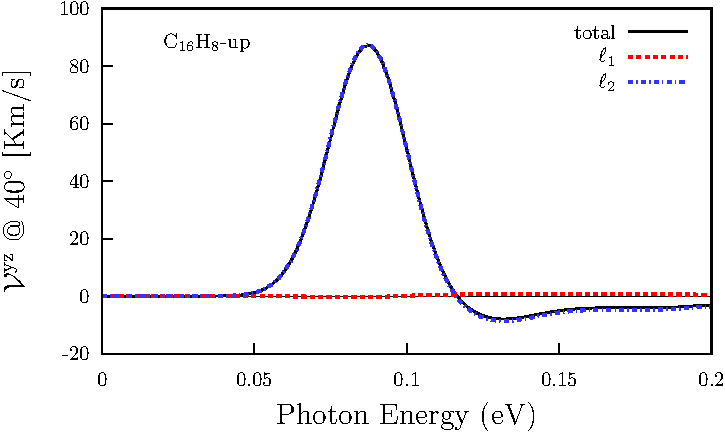
\includegraphics[width=\linewidth]{upplots/up-vyz-layers-1}}
    \\
    \subfigure[\ \label{fig:up-vyz-lay-2}]
    {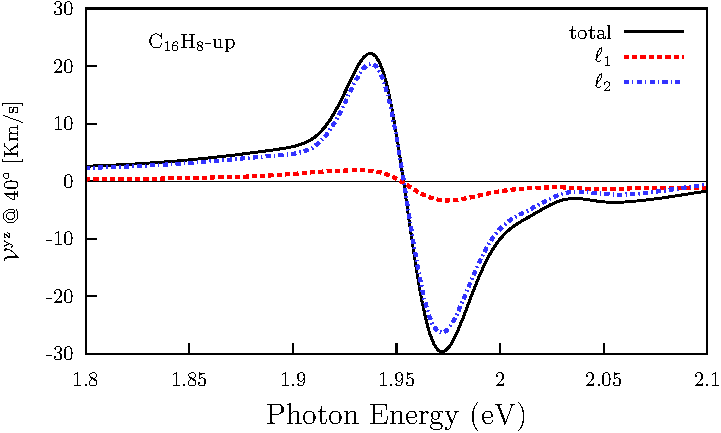
\includegraphics[width=\linewidth]{upplots/up-vyz-layers-2}}
    \caption{Layer-by-layer contribution of $\mathcal{V}^{\mathrm{yz}}$ for the
     \emph{up} structure.}
    \label{fig:up-vyz-lay}
\end{figure}

From the bottom frames of Figs. \ref{fig:up-vab-comp-rtp-1} and 
% 
\ref{fig:up-vab-comp-rtp-2} we can see that for the \emph{up} structure again
the most intense component of $|\mathcal{V}^{\mathrm{x}}|$ and
$|\mathcal{V}^{\mathrm{y}}|$ corresponds to $\mathcal{V}^{\mathrm{yz}}$ which
has a value of 87.2\,Km/s for an energy incident beam of 0.088\,eV and
-29.7\,Km/s for an energy incident beam of 1.972\,eV. This component and the
corresponding layer by layer contribution is depicted in Fig. 
\ref{fig:up-vyz-lay}s.
% 
From this figure we have that for the energy range from 0\,eV to 0.2\,eV the
response comes from the second layer composed by carbon atoms presented in Tab.
\ref{tab:up-unitcell} and denoted by the number 2 in Fig. \ref{fig:up-struc}. In
the other hand, the response for the energy range from 1.8\,eV to 2.1\,eV almost
all the response comes from the carbon atoms having a leaser contribution from
the hydrogen layer.
% %%%%%%%%%%%%%%%%
% %% Description of ALT layer |V^{yz}|
% %% files:  v.sm_0.03_yz_14452_65-spin_scissor_0_Nc_32_ang_145
% %%         calv.sm_0.03_yz_14452_1_65-spin_scissor_0_Nc_32_ang_145
% %%         calv.sm_0.03_yz_14452_2_65-spin_scissor_0_Nc_32_ang_145
% %%         calv.sm_0.03_yz_14452_3_65-spin_scissor_0_Nc_32_ang_145
% %%         calv.sm_0.03_yz_14452_4_65-spin_scissor_0_Nc_32_ang_145
% %%         calv.sm_0.03_yz_14452_5_65-spin_scissor_0_Nc_32_ang_145
% %%         calv.sm_0.03_yz_14452_6_65-spin_scissor_0_Nc_32_ang_145
% %%         alt-plots/alt-vab-layers.gp
% %%%%%%%%%%%%%%%%
From the bottom frames of Fig. \ref{fig:alt-vab-comp-rtp} we can see that for
the \emph{alt} structure the most intense component of
$|\mathcal{V}^{\mathrm{x}}|$ and $|\mathcal{V}^{\mathrm{y}}|$ corresponds to
$\mathcal{V}^{\mathrm{yz}}$ which has a value of -40.2\,Km/s for an
energy incident beam of 0.72\,eV. This component and the corresponding layer by
layer contribution is depicted in Fig. \ref{fig:alt-vyz-lay}. From this figure
we have that for the energy range from 0.70\,eV to 0.74\,eV the fifth and sixth
layers corresponding to the bottom carbon and hydrogen numbered with 5 and 6 in
Fig. \ref{fig:alt-struc} have contributions in opposite direction than the other
4 layers resulting in a total response $\mathcal{V}^{\mathrm{yz}}= -40.2$\,Km/s
for an incoming beam energy of 0.72\,eV. In the other hand, for the energy range
from 0.88\,eV to 0.95\,eV the response for the all six layers the responses are
in the same direction resulting in a total response
$\mathcal{V}^{\mathrm{yz}}=-32.89$\,Km/s for an incoming beam with energy of
0.912\,eV.
\begin{figure}[b]
    \centering
    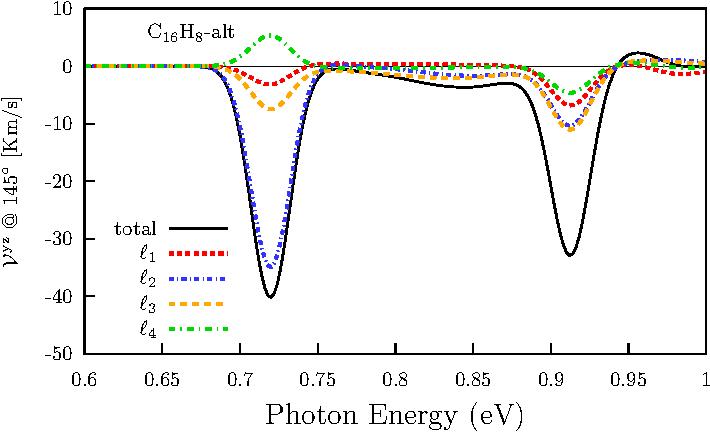
\includegraphics[width=\linewidth]{altplots/alt-vyz-layers}
    \caption{Layer-by-layer contribution of $\mathcal{V}^{\mathrm{yz}}$ for the
     \emph{alt} structure.}
    \label{fig:alt-vyz-lay}
\end{figure}




\bibliography{article.bib}

\end{document}

















